\section{Templates}




\subsection{Boat}
The boat template as the name infers is a model of the real boat. The boat is capable of carrying at most two persons and most have at least one adult to handle the boat. From the initial state, called still, the only possible edge is to listen 
\begin{figure}%
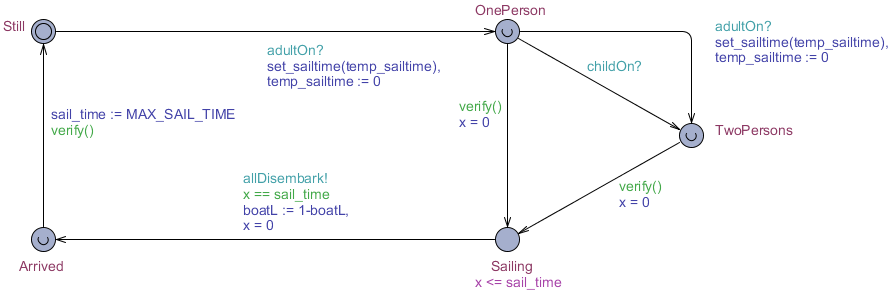
\includegraphics[width=\columnwidth]{pictures/boat.png}%
\caption{}%
\label{}%
\end{figure}
















\section{Person}
\begin{figure}%
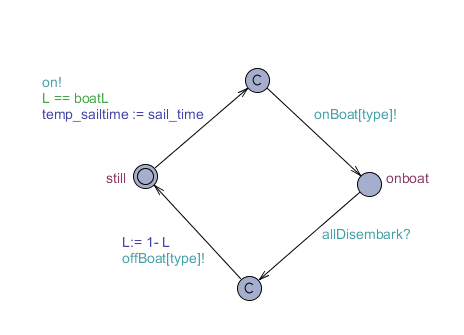
\includegraphics[width=\columnwidth]{pictures/person.png}%
\caption{}%
\label{}%
\end{figure}



















\section{Observer}
The purpose of the observer is to keep track of where the diffent persons are located. It maintains the following two arrays:
\begin{itemize}
	\item[left] Is an array with a list of all the person on the original shore(left)
	\item[right] Contains a list of all person on the taget shore(right)
\end{itemize}

On figure \ref{fig:observer} the model of the observer is displayed. There exist one instant of observer, when a person broadcasts onBoat or offBoat the observer listen and relativly run the function updateOn or updateOff. 
The updateOn and updateOff functions recives a personType as input. updateOn removeds the personType form the relevant array. updateOff adds the given personType from the relevant array. This implyes that we do not destinguesh between the different person but only requirer that they are of a given type. The implemtation of this gives rise to stage space explotion, e.g. a boy and the man is located on the left shore, the array containing this information can either be \{boy,man\} or \{man,boy\} which of course is equivalent but uppaal regards this as two diffent stats. To solve this we implemented a sorting funcitons to insure that left and right array are always sorted and thus avoid stage space explotion.
  




\begin{figure}%
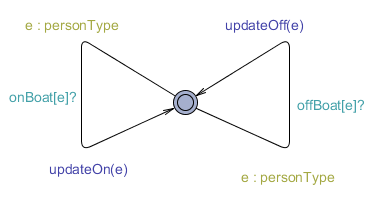
\includegraphics[width=\columnwidth]{pictures/observer.png}%
\caption{}%
\label{fig:observer}%
\end{figure}




























\section{Observer}